%%%%%%%%%%%%%%%%%%%%%%%%%%%%%%%%%%%%%%%%%%%%%%%%%%%%%%%%%%%%%%%%%%%%%%%%%%%%%%%
%%%%%%%%%%%%%%%%%%%%%%%%%%%%%%%%%%%%%%%%%%%%%%%%%%%%%%%%%%%%%%%%%%%%%%%%%%%%%%%
%%%%%%%%%%%%%%%%%%%%%%%%%%%%%%%%%%%%%%%%%%%%%%%%%%%%%%%%%%%%%%%%%%%%%%%%%%%%%%%
%
\begin{figure}[h]
\centering
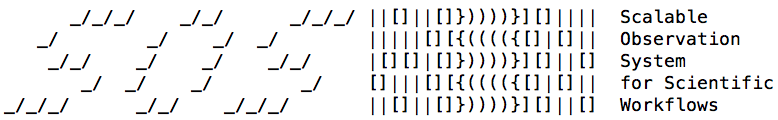
\includegraphics[width=\columnwidth]{images/sosflow_masthead.png}
\label{fig_masthead}
\end{figure}
%
%%%%%%%%%%%%%%%%%%%%%%%%%%%%%%%%%%%%%%%%%%%%%%%%%%%%%%%%%%%%%%%%%%%%%%%%%%%%%%%
%%%%%%%%%%%%%%%%%%%%%%%%%%%%%%%%%%%%%%%%%%%%%%%%%%%%%%%%%%%%%%%%%%%%%%%%%%%%%%%
%%%%%%%%%%%%%%%%%%%%%%%%%%%%%%%%%%%%%%%%%%%%%%%%%%%%%%%%%%%%%%%%%%%%%%%%%%%%%%%
\section{Introduction}
%
\par
%
Modern clusters for parallel computing are complex environments and
the high-performance applications that run on them do so often with
little insight about their or the system's behavior.
%
This is not to say that information is unavailable.  After all,
sophisticated parallel measurement systems can capture performance and
power data for characterization, analysis, and tuning purposes, but
the infrastructure for observation of these systems is not intended
for general use.
%
Rather, it is specialized for certain types of performance information
and typically does not allow online processing.
%
Other information sources of interest might include the
operating system (OS), network hardware, runtime services, or the
parallel application itself.
%
\par
%
Cluster monitoring systems like Ganglia \cite{massie2004ganglia} or
Nagios \cite{katsaros2011building} collect and process data about the
performance and health of cluster-wide resources, but do not provide
sufficient fidelity to capture the complex interplay between
applications competing for shared resources.
%
In contrast, the Lightweight Distributed Metric Service
\cite{agelastos2014lightweight} (LDMS) attempts to capture system data
continuously to obtain insight into behavioral characteristics of
individual applications with respect to their resource utilization.
%
However, neither of these provides a framework that can be configured
with and used directly by the application, nor allow for semantic
encoding of multiple observation sources.
%
\par
%
Our general interest is in parallel application monitoring: the
observation, introspection, and possible adaptation of an application
during its execution.
%
Application monitoring has several requirements.
%
Because information could come from different sources and be used for
different purposes, it is important to have a flexible means for
information to be provided from both the application and the system
environment.
%
Because information will need to be processed online, it is important
to enable analysis in situ with the application.
%
Because analysis can result in application feedback, query and control
interfaces are required, again to both the application and the system.
%
There exists no general purpose infrastructure that can be programmed,
configured, and launched with the application to provide the
integrated observation, introspection, and adaptation support
required.
%
\par
%
This paper presents the \textit{Scalable Observation System (SOS)} for
integrated application monitoring.
%
A working implementation of SOS is contributed as a part of this
research effort, the \textit{SOSflow} runtime.
%
The SOSflow platform demonstrates all of the essential characteristics
of the SOS model, showing the scalability and flexibility inherent to
SOS with its support for observation, introspection, feedback, and
control of scientific workflows.
%
The SOS design emphasizes a semantic data model with distributed
information management and structured query and access.
%
A dynamic database architecture is used in SOS to support aggregation
of streaming observations from multiple sources.
%
SOS provides interfaces for sources of information to encode data along
with its context and meaning.
%
Interfaces are also provided for in situ analytics to acquire
information and send back results for application actuators.
%
SOS launches with the application, runs along side it, and can acquire
its own resources for scalable data collection and processing.
%


\subsection{Scientific Workflows} %-------------------------------------------%
%
Scientific workflows feature two or more components that are coupled
together, operating over shared information to produce a cumulative
result.
%
These components can be instantiated as lightweight threads belonging
to a single process, or they may execute concurrently as independent
processes.
%
Components of workflows may be functionally isolated from of each
other or synchronously coupled and co-dependent.
%
Parts of workflows may even be dynamically instantiated and
terminated.
%
The computational profile of a workflow can change during the course
of its execution.
%
Any general solution for monitoring workflows will need to be capable
of contextualizing the information processesed by any single
component, in a scope that can contain and adequatelty contexualize
the union of all other component scopes.
%
\par
%
This research contributes a general solution to the monitoring
challenges posed by scientific workflows.
%
To address the general case, SOSflow operates independently of any
given component and the technology employed to couple components into
a workflow.
%
SOSflow's behavior is not bound by the nature of the workflows it
operates alongside, and by design SOSflow is not limited to a specific
scale or execution environment.
%
%This particular research effort focuses on three aspects of SOSflow:
%
%\begin{itemize}
%\item \textbf{On-line Ca}
%\item \textbf{Scalable Architecture}
%\item \textbf{Global Information Space}
%\end{itemize}
%
\par
%
No extant software system adequately expressed all of the properties
required for the SOSflow model, motivating its development and
contribution as a novel software artifact.
%
SOSflow provides a flexible research platform for investigating the
properties of existing and future scientific workflows, supporting
both current and future scales of execution.
%
\subsection{Application Perspective} %----------------------------------------%
%
%
\subsection{System Perspective} %---------------------------------------------%
%
%
\subsection{Tool Perspective} %-----------------------------------------------%
%
%
\subsection{Exascale Measurement Challenge} %---------------------------------%
%
%
\subsection{Summary} %--------------------------------------------------------%
%
%



%%%
%%%  EOF
%%%

